\documentclass[11pt]{article}
\usepackage{html}
\usepackage{psfig}
\usepackage{makeidx}
\usepackage{nomencl}
\oddsidemargin  -0.1in   %  Note that \oddsidemargin = \evensidemargin
\evensidemargin -0.1in

\topmargin -55pt         %    Nominal distance from top of page to top
                         %    of box containing running head.
\headheight 12pt         %    Height of box containing running head.
\headsep 25pt            %    Space between running head and text.
\footskip 60pt           %    Distance from baseline of box containing


\textheight 9.125in        % Height of text (including footnotes and
                         % figures, excluding running head and foot).
\textwidth 6.75in         % Width of text line.
                         % For two-column mode:

\textheight 9.125in        % Height of text (including footnotes and
                         % figures, excluding running head and foot).
\textwidth 6.75in         % Width of text line.
                         % For two-column mode:
\renewcommand{\baselinestretch}{1.2}
\renewcommand{\nomname}{Glossary}
\makeindex\makeglossary

\title{TinyDB:  In-Network Query Processing in TinyOS}
% \author{Sam Madden and his Band of Merry Old Men}
\date{}


\begin{document}
\pagenumbering{arabic}
\pagestyle{myheadings}
\markright{{\bf TinyDB\index{TinyDB} Documentation. }}

\maketitle
\thispagestyle{empty}

\section{Introduction}

TinyDB\index{TinyDB} is a query processing system for extracting
information from a network of
\htmladdnormallink{TinyOS}{http://webs.cs.berkeley.edu/tos}
sensors.\index{TinyOS}\index{sensor} Unlike existing
solutions for data processing in TinyOS\index{TinyOS},
TinyDB\index{TinyDB} does not require you to write embedded C\index{C}
code for sensors\index{sensor}\index{embedded}.
Instead, TinyDB\index{TinyDB} provides a
simple, SQL\index{SQL}-like interface to specify the data you want to
extract, along with additional parameters, like the rate at which data
should be refreshed -- much as you would pose queries against a
traditional database.  
Given a query specifying your data interests,
TinyDB\index{TinyDB} collects that data from motes\index{mote} in the
environment, filter\index{filter}s it, aggregates\index{aggregate} it together, and routes it out to
a PC.  TinyDB\index{TinyDB} does this via power-efficient in-network\index{in-network}
processing algorithms.

To use TinyDB\index{TinyDB}, you install its TinyOS\index{TinyOS} components\index{component} onto
each mote\index{mote} in your sensor\index{sensor} network. (TinyDB\index{TinyDB}'s components\index{component} can co-exist
with other components\index{component}, although they can place extensive demands on
the memory and radio resources of the mote\index{mote}.)  TinyDB\index{TinyDB} provides a simple
Java\index{Java} API\index{API} for writing PC applications that query and extract data from
the network; it also comes with a simple graphical query-builder and
result display that uses the API\index{API}.

The primary goal of TinyDB\index{TinyDB} is to make your life as a programmer
significantly easier, and allow data-driven applications to be
developed and deployed {\em much} more quickly than what is currently
possible.  TinyDB\index{TinyDB} frees you from the burden of writing low-level code
for sensor\index{sensor} devices, including the (very tricky) sensor network\index{sensor network}
interfaces.  Some of the management features of TinyDB\index{TinyDB} include:

\begin{itemize}
\item {\it Network Topology\index{topology}}: TinyDB\index{TinyDB} manages the underlying radio network by tracking
neighbors\index{neighbor}, maintaining routing\index{routing} tables\index{table}, and ensuring that every mote\index{mote} in the
network can efficiently and (relatively) reliably deliver its data to the user.
\item {\it Multiple Queries}: TinyDB\index{TinyDB} allows multiple queries to be run on the same
set of motes\index{mote} at the same time.  Queries can have different sample\index{sample} rates and
access different sensor\index{sensor} types, and TinyDB\index{TinyDB} efficiently shares work between
queries when possible.
\item {\it Incremental Deployment via Query Sharing}: To expand your
TinyDB\index{TinyDB} sensor network\index{sensor network}, you simply download\index{download} the standard TinyDB\index{TinyDB} code to
new motes\index{mote}, and TinyDB\index{TinyDB} does the rest.  TinyDB\index{TinyDB} motes\index{mote} share queries with
each other: when a mote\index{mote} hears a network message for a query that it is
not yet running, it automatically asks the sender of that data for a
copy of the query, and begins running it.  No programming or
configuration of the new motes\index{mote} is required beyond installing TinyDB\index{TinyDB}.
\end{itemize}

This document serves a number of purposes.  The first sections are
targeted at the sensor\index{sensor} application programmer, and include a basic
overview of the TinyDB\index{TinyDB} system architecture, and a QuickStart guide to
using the TinyDB\index{TinyDB} system, its query language and APIs\index{API}.  The remaining
sections are targeted at readers who want to extend the TinyDB\index{TinyDB} system
itself.  They describe the TinyDB\index{TinyDB} software components\index{component}, highlighting
places where the system could be profitably extended.

\subsection{System Overview}

This section provides a high level overview of the architecture of the TinyDB\index{TinyDB} software.  It
is designed to be accessible to users of the TinyDB\index{TinyDB} system who are not interested in
the technical details of the system's implementation.  A detailed
description of the TinyDB\index{TinyDB} software design
is reserved for section \ref{sec:inside}.  

We begin with a short description of a typical use-case for TinyDB\index{TinyDB}.  Imagine that Mary
wishes to locate a conference room in her sensor\index{sensor}-equipped building that is currently not in use, and
that an application to perform this task has not already been built.
The motes\index{mote} in Mary's
building have a sensor\index{sensor} board\index{board} with light sensors\index{sensor} and microphones and have been programmed with
a room number.  Mary decides that her application
should declare a room {\it in-use} when the average light reading of all the sensors\index{sensor} in a room
are above $l$ and when the average volume is above $v$.  Mary wants her application to 
refresh this occupancy information every 5 minutes.  Without TinyDB\index{TinyDB}, Mary
would have to write several hundred lines of custom embedded C\index{C}
code~\index{embedded} to collect information
from all the motes\index{mote} in a room, coordinate the communication of readings
across sensors\index{sensor},
aggregate\index{aggregate} these readings together to compute the average light
and volume, and then forward that information from within the sensor network\index{sensor network} to the PC where
the application is running.  She would then have to download\index{download} her compile\index{compile}d
program to each of the motes\index{mote} in the room.  Instead, if the motes\index{mote} in Mary's building are running TinyDB\index{TinyDB},
she can simply pose the following SQL\index{SQL}
query to identify the rooms that are currently in-use:

\noindent{\tt \hspace{.5in}SELECT AVG(light), AVG(volume) \\
\hspace*{.5in}FROM sensors\index{sensor} \\
\hspace*{.5in}GROUP BY roomno \\
\hspace*{.5in}HAVING AVG(light) > $l$ AND AVG(volume) > $v$ \\
\hspace*{.5in}EPOCH DURATION 5min
}

\noindent TinyDB\index{TinyDB} translates this query into an efficient
execution plan\index{query plan} which
delivers the set of occupied rooms every 5 minutes\index{epoch}.  Mary simply inputs this query
into a GUI\index{GUI} -- she writes no C\index{C} code and is freed from 
concerns about how to install her code, how to propagate results across
multiple network hops\index{hop}\index{multi-hop} to the root\index{root} of the network, how to power down sensors\index{sensor} 
during the time when they are not collecting and reporting data, and many other
difficulties associated with sensor-network\index{sensor network} programming.

We discuss the inner workings of TinyDB\index{TinyDB} on such queries in
Section \ref{sec:inside} below.  In the remainder of this section, we
present a high-level overview of the components\index{component} of TinyDB\index{TinyDB}.  The system
can be broadly classified into two subsystems:

\begin{enumerate}
\item \underline{Sensor Network\index{sensor network} Software:}  This is the heart of TinyDB\index{TinyDB}, although most users of
the system should never have to modify this code.  It runs on each
mote\index{mote} in the network, and consists of several major pieces:
\begin{itemize}
\item {\it Sensor\index{sensor} Catalog\index{catalog} and Schema\index{schema} Manager}:  The catalog\index{catalog} is responsible for tracking the
set of {\it attributes\index{attribute}}, or types of readings (e.g. light, voltage, parent\index{parent} node\index{node}, etc.) available
on each sensor\index{sensor}.  In general, this list is not identical for each sensor\index{sensor}:  networks may consist
of heterogeneous collections of devices.  (See
Section~\ref{sec:catalog} for details.)

\item {\it Query Processor\index{query processor}}:  The main component\index{component} of TinyDB\index{TinyDB} consists of a small query processor\index{query processor}.  
The query processor\index{query processor} uses the catalog\index{catalog} the fetch the values of local attributes\index{attribute}, receives sensor\index{sensor}
readings from neighboring\index{neighbor} nodes\index{node} over the radio, combines and aggregates\index{aggregate} these values together,
filters\index{filter} out undesired data, and outputs values to
parent\index{parent}s.  (See Section~\ref{sec:qp} for details.)

\item {\it Memory Manager}:  TinyDB\index{TinyDB} extends TinyOS\index{TinyOS} with a small, handle-based\index{handle}
  dynamic memory manager.  (See Section~\ref{sec:tinyalloc} for details.)

\item {\it Network Topology\index{topology} Manager}: TinyDB\index{TinyDB} manages the connectivity
  of motes\index{mote} in the network, to efficiently route data and subquery
  results through the network.  (See Section~\ref{sec:tinydbnetwork}
  for details.)
\end{itemize}
\item \underline{Java\index{Java}-based Client\index{client} Interface:}
A network of TinyDB\index{TinyDB} motes\index{mote} is accessed from a connected PC through the
{\em TinyDB\index{TinyDB} client\index{client} interface}, which consists
of a set of Java\index{Java} classes and applications.  These classes are all stored in the {\tt nest/tools/tinyos/tinydb} 
package in the source tree.  The specific classes are described in Section \ref{sec:runningqueries};  major
classes include:
\begin{itemize}
\item Classes to extract information about the attributes\index{attribute} and capabilities of devices
\item Classes to build and transmit queries
\item Classes to receive and parse query results
\item A GUI\index{GUI} to construct queries
\item A graph and table\index{table} GUI\index{GUI} to display individual sensor\index{sensor} results
\item An application that use queries as an interface on top of a network of sensors\index{sensor}
\end{itemize}
\end{enumerate}

\subsection{Installation and Requirements}
\marginpar{Should be replaced with a thorough, step-by-step ``Getting Started'' section.}
TinyDB\index{TinyDB} requires a basic TinyOS\index{TinyOS} installation, with a working Java\index{Java}
installation (and javax.comm library).  For installation instructions
on TinyOS\index{TinyOS}, see the \htmladdnormallink{TinyOS\index{TinyOS} web
page}{http://webs.cs.berkeley.edu/tos}.

TinyDB\index{TinyDB} is not currently a part of an official TinyOS\index{TinyOS} release.  To obtain
the code, you will need to check out a recent version from CVS;  see the
\htmladdnormallink{TinyOS\index{TinyOS} CVS Page}{http://sf.net/cvs/?group_id=28656}
for instructions on using CVS.

In addition to the standard distribution, the following files are a
part of the TinyDB\index{TinyDB} distribution:

\renewcommand{\baselinestretch}{.9}\rm
\begin{itemize}
\item {\tt nest/apps/tinydbtest}
\begin{itemize}
\item {\tt /TUPLE\_ROUTER.\{c,comp\}}
\item {\tt /TINYDB.desc}
\item {\tt /TINYDB\_NETWORK.\{c,comp\}}
\item {\tt /TUPLE.\{c,comp\}}
\item {\tt /ATTR.\{c,comp\}}
\item {\tt /QUERY\_RESULT.\{c,comp\}}
\item {\tt /AGG\_OPERATOR.\{c,comp\}}
\item {\tt /SELECT\_OPERATOR.\{c,comp\}}
\item {\tt /MAGNET.\{c,comp\}}
\end{itemize}
\item {\tt nest/tos/include}
\begin{itemize}
\item {\tt /TinyDB.h}
\item {\tt /TinyDBError.h}
\item {\tt /SchemaAPI.h}
\item {\tt /SchemaError.h}
\end{itemize}
\item {\tt nest/tos/shared}
\begin{itemize}
\item {\tt /SCHEMA.\{c,comp\}}
\item {\tt /TINY\_ALLOC.\{c,comp\}}
\end{itemize}
\item {\tt nest/tools/net/tinyos/tinydb}
\begin{itemize}
\item {\tt AggExpr.java}
\item {\tt AggOp.java}
\item {\tt Catalog.java}
\item {\tt CmdFrame.java}
\item {\tt CommandMsgs.java}
\item {\tt MagnetFrame.java}
\item {\tt QueryExpr.java}
\item {\tt QueryField.java}
\item {\tt QueryListener.java}
\item {\tt QueryResult.java}
\item {\tt ResultFrame.java}
\item {\tt ResultGraph.java}
\item {\tt ResultListener.java}
\item {\tt SelExpr.java}
\item {\tt SelOp.java}
\item {\tt TinyDBCmd.java}
\item {\tt TinyDBMain.java}
\item {\tt TinyDBNetwork.java}
\item {\tt TinyDBQuery.java}
\end{itemize}
\end{itemize}
\renewcommand{\baselinestretch}{1.2}\rm

To verify that your installation is working properly, try the following:

\begin{enumerate}
\item Compile\index{compile} and install TinyDB\index{TinyDB} on the mote\index{mote}.  To do this, connect the mote\index{mote} to
the programming board\index{board}, then type the following:
\begin{itemize}
\item {\tt cd nest/apps/tinydbtest/}
\item {\tt make mica}
\item {\tt make mica install}
\end{itemize}
If this fails, verify that your installation works (see the instructions on the web
site), and that you have all of the TinyDB\index{TinyDB} files listed above.
\item Compile\index{compile} and run the TinyDB\index{TinyDB}Main java\index{Java} classes.  To do this, type the following:
\begin{itemize}
\item {\tt cd nest/tools}
\item {\tt javac net/tinyos/tinydb/*.java}
\item {\tt java net.tinyos.tinydb.TinyDB\index{TinyDB}Main}
\end{itemize}
\end{enumerate}
You may see warnings about ``deprecated classes'' when {\tt javac}
runs.  These are OK, and you can ignore them.  
You should see the TinyDB\index{TinyDB} control panel and query interface appear.

Once you have a working installation of these files, continue on to the next section
to learn how to run queries with TinyDB\index{TinyDB}.

\section{Quick Start:  Running Queries with TinyDB\index{TinyDB}} \label{sec:runningqueries}

In this section, you will learn how to set up a network of TinyDB\index{TinyDB} motes\index{mote}, inject a query
into the network, and collect the results of the query.  

\subsection{Setting up a Network of TinyDB\index{TinyDB} motes\index{mote}}

The first step is to program a number
of motes\index{mote} with the TinyDB\index{TinyDB} software.  Each of these motes\index{mote} must have a unique id;  recall that,
in TinyOS\index{TinyOS}, you can set the ID of a mote\index{mote} when running {\tt make install} by appending {\tt .node\index{node}id}
-- for example, to program a TinyDB\index{TinyDB} mote\index{mote} at ID 2, you would type:

\begin{itemize}
\item {\tt cd nest/apps/tinydbtest/}
\item {\tt make mica install.2}
\end{itemize}

\noindent To run TinyDB\index{TinyDB}, you will need at least two motes\index{mote}:  one to act as the basestation, and one
or more to distribute and run queries over.  All motes\index{mote}, including the basestation, run the same
{\tt tinydbtest} application, however, {\it the basestation must be set to ID 0.}  

After programming your motes\index{mote}, connect the programming board\index{board} to your computer (via the serial
port\index{serial}), and place the basestation in the programming board\index{board}.  Turn on all of the motes\index{mote}.

\subsection{Running the TinyDB\index{TinyDB}Main GUI\index{GUI}}

The TinyDB\index{TinyDB}Main Java\index{Java} application provides a graphical interface for distributing queries 
over motes\index{mote} and collecting data from them.  To run this application, type:

\begin{itemize}
\item {\tt cd nest/tools}
\item {\tt javac net/tinyos/tinydb/*.java}
\item {\tt java net.tinyos.tinydb.TinyDB\index{TinyDB}Main}
\end{itemize}

Two windows should appear;  one, the {\it command} window (Figure \ref{fig:command}),
 allows you to send a variety of control commands to the motes\index{mote}.  The other, the {\it query} window
(Figure \ref{fig:query}),
allows you to build and send queries into the network.  We focus on the operation of the
query window in this section.

\begin{figure}[ht]
\psfig{figure=querywin.eps,width=4in}
\caption{The Query Window}
\label{fig:query}
\end{figure}
\par

\begin{figure}[ht]
\psfig{figure=commandwin.eps,width=1.5in}
\caption{The Command Window}
\label{fig:command}
\end{figure}
\par


\subsection{Queries in TinyDB\index{TinyDB}}
\label{sec:queries}
Queries in TinyDB\index{TinyDB} consist of a set of attributes\index{attribute} (e.g. light, temperature), a set of 
{\it selection\index{selection} predicates\index{predicate}}, and a set of {\it aggregation\index{aggregation} predicates\index{predicate}}.  
attributes\index{attribute} 
Currently, aggregation\index{aggregation} predicates\index{predicate} are {\it spatial}\index{spatial} -- that is,
they combine values between sensors\index{sensor} in the environment.  {\it Temporal}\index{temporal} aggregates\index{aggregate}, that combine
readings from the same sensor\index{sensor} over several time periods, are not supported in the current
release.

Queries can also contain {\it selection\index{selection} predicates\index{predicate}} and {\it group-by\index{Group By} clauses}.  

\subsubsection{TinyDB\index{TinyDB} SQL\index{SQL} vs. Standard
  SQL\index{SQL}}
{\bf FILL ME IN!}

\section{Developing For TinyDB\index{TinyDB}: Java\index{Java} API\index{API}}
A network of motes\index{mote} running TinyDB\index{TinyDB} is relatively uninteresting without
an external program to send in queries and receive responses.  TinyDB\index{TinyDB}
provides a Java\index{Java} API\index{API} for building such programs, and also includes a
sample\index{sample} program that uses that API\index{API} to provide a graphical query
builder, and a graphical result display.

We begin with an overview of the API\index{API}, and go on to an overview of the
sample\index{sample} program that exercises the API\index{API}.

\subsection{The TinyDB\index{TinyDB} Java\index{Java} API\index{API}}
The API\index{API} contains a number of objects:
\begin{itemize}
\item {\tt TinyDB\index{TinyDB}Network}: This object is the main interface to a
  network of motes\index{mote}.  It is responsible for injecting new queries into
  the network ({\tt sendQuery()}), for cancelling queries ({\tt
  abortQuery()}), and for providing results from the network to
  multiple query ``listeners''\index{listener}.  Only one instance\index{instance} of the {\tt
  TinyDB\index{TinyDB}Network} object needs to be allocated for a network; that
  instance can manage multiple ongoing queries, and multiple
  listeners.  Each query's output can be sent to multiple listeners,
  and each listener can listen either to a single query, or to all
  queries.
  
  Internally, the object maintains a list of live queries, and three
  sets of listeners\index{listener}:
  \begin{enumerate}
	\item {\tt processedListeners} are signed up for a specific query
    ID, and get a stream of final (``processed''\index{processed}) answer tuples\index{tuple} for
    that query.
	\item {\tt qidListeners} are signed up for a specific query ID,
    and get copies of all messages that arrive for that query.  These
    messages may not be final query answers.  They may be individual
    attributes\index{attribute} from an answer tuple\index{tuple}, or unaggregated\index{aggregate} sub-result
    tuples\index{tuple}.
	\item  {\tt listeners} are signed up to receive a copy of all
    unprocessed messages for {\em all} queries.  
  \end{enumerate}
  The various listeners can be added or deleted to the object on the
  fly via {\tt addResultListener()} and {\tt removeResultListener()}
  -- note that different arguments to the {\tt addResultListener}
  method result in one of the 3 different kinds of listeners above.

  The {\tt TinyDB\index{TinyDB}Network} object handles all incoming
  AM\index{Active Messages (AM)}\glossary{AM} messages from the
  serial port\index{serial}, and dispatches copies of them to the {\tt listeners}
  and {\tt qidListeners} accordingly.  It also processes the messages
  to generate result tuples\index{tuple} (via {\tt QueryResult.MergeQueryResult()})
  and sends them to {\tt processedListeners} accordingly.  As part of
  processing results, it maintains info on epochs\index{epoch} to make sure that
  the epoch\index{epoch} semantics\index{semantics} of the results are correct.

  Internally, the {\tt TinyDB\index{TinyDB}Network} object also has a background thread
  that participates in the sensor network's\index{sensor network} routing\index{routing} algorithms.  It
  periodically sends information down the routing\index{routing} tree, so that
  children know to choose the root\index{root} as a parent\index{parent}, and so that children
  can decide how to share the timeslots\index{timeslot} in an epoch\index{epoch}.  {\bf Note
  dependency here: programmers wanting to hack the topology\index{topology} code need
  to hack here too.}

\item {\tt TinyDB\index{TinyDB}Query}: This is a Java\index{Java} data structure representing a
    query running (or to be run) on a set of motes\index{mote}.
    
    Queries consist of:
    \begin{itemize}
    \item a list of attributes\index{attribute} to select
    \item a list of expressions\index{expression} over those fields, where an expression\index{expression}
    is
      \begin{itemize}
      \item a filter\index{filter} that discards readings that do not match a
      boolean expression\index{expression}
      \item an aggregate\index{aggregate} that combines local readings with readings from
        neighbors\index{neighbor}, and optionally includes a GROUP BY\index{Group By} column.  {\bf
        (Hack: GROUP BY\index{Group By} columns can optionally be bit-shifted before
        the grouping\index{group} happens, to make for fewer groups\index{group} (buckets) on a
        dense domain.  This is called ``attenuation\index{attenuation}'' in the API\index{API}.)}
        {\bf (Limitation: GROUP BY\index{Group By} can currently only be done on a
        single attribute\index{attribute}, and not on multiple
        attribute and/or expressions\index{expression}.)} 
      \end{itemize}
    \item An SQL\index{SQL} string.  This currently has no specific relationship
    to the fields or expressions\index{expression}, and is largely ignored in the
    current code.  It is for the future use of a parser, which will
    some day squirrel its query away here for reference after setting
    up the fields and expressions\index{expression}.
    \end{itemize}

   In addition to allowing a query to be built, this class includes
   handy methods to generate specific radio messages for the query,
   which {\tt TinyDB\index{TinyDB}Network} can use to distribute the query over the
   network, or to abort the query.

   It also includes a support routine for printing the query result
   schema\index{schema}.

\item {\tt QueryResult}: This object accepts a query result in the
    form of an array of bytes read off the network, parses the results
    based on a query specification, and provides a number of utility
    routines to read the values back.  It also provides the {\tt
    mergeQueryResult} functionality for {\tt processedListeners}\index{listener}.
    This does concatenation of multiple aggs as separate attributes of
    a single result tuple, and finalizes aggregates\index{aggregate}, by
    combining data from multiple sensors\index{sensor} talk to 
    the API\index{API}.)

\item {\tt AggOp}: This provides the code for the aggregation\index{aggregation}
  operators SUM, MIN, MAX, and AVERAGE.  It includes representation
  issues (internal network codes for the various ops, and code for
  pretty-printing), and also the logic for performing final merges for
  each aggregate\index{aggregate} as part of {\tt QueryResult:MergeQueryResult()}.
  {\bf This is another place you need to touch if you want to add your
  own aggs.}

\item {\tt SelOp}: This provides the logic for selection\index{selection} predicates\index{predicate}.
  Currently this includes representations for simple arithmetic
  comparisons (internal network codes for the arithmetic comparators,
  and pretty-printing.)

\item {\tt Catalog\index{catalog}:} This object provides a very (very!) simple parser
  for a catalog\index{catalog} file -- it reads in the file, and after parsing it
  provides a list of attributes\index{attribute}.

\item {\tt CommandMsgs}: This is a class with static functions to
    generate message arrays that can be used to invoke commands on Db
    motes\index{mote}.

\end{itemize}
\subsection{The TinyDB\index{TinyDB} Demo Application}
The TinyDB\index{TinyDB} application allows users to interactively specify queries
and see results.  It also serves as an example of an application that
uses the TinyDB\index{TinyDB} API\index{API}.  As with traditional database systems, it is
expected that many programmers will want to embed queries within more
specialized application code.  Such programmers can look at the TinyDB\index{TinyDB}
application for an example of how this is done.

The TinyDB\index{TinyDB} application consists of only a few objects:
\begin{itemize}
\item {\tt TinyDB\index{TinyDB}Main}: This is the main loop for the application.  It
  opens an {\em Active Message (AM)}\index{Active Messages (AM)} connection to
  the Serial Port\index{serial} (``COM1''\index{COM1}), and uses it to initialize a {\tt
  TinyDB\index{TinyDB}Network} object.  It
  allocates the GUI\index{GUI} objects {\tt CmdFrame} and {\tt QueryFrame} for
  the application, which issue queries and in turn generate visualizations
  of results.  There are also some simple wrapper routines for
  the {\tt TinyDbNetwork} methods to add and remove queries from listeners.

\item {\tt CmdFrame}: This is a simple GUI\index{GUI} for sending TinyDB\index{TinyDB} commands
  (from the {\tt CommandMsgs} API\index{API} object) into the network.  See Figure~\ref{fig:command}.

\item {\tt QueryFrame}: A graphical query builder to construct a valid
  {\tt TinyDB\index{TinyDB}Query} object and send it into the network via {\tt
  TinyDB\index{TinyDB}Network.sendQuery()} (Figure~\ref{fig:query}.)  In addition to
  allowing users to specify ad hoc queries\index{ad hoc}, it provides a button to
  send off two pre-prepared queries that have special visualizations:
  \begin{enumerate}
  \item A visualization of the network topology\index{topology}, which is extracted
  from the network via a standard TinyDB\index{TinyDB} query. (The ``Display
  Topology'' button in Figure~\ref{fig:query}.)
  \item A visualization of magnetometers laid out in a fixed $x \times
  y$ grid. This is an example of simple demo application that can run on
  TinyDB:  in this case, TinyDB is used to identify sensors with 
  magnetometer readings greather than some threshold to detect metallic
  objects moving through a grid of motes. It is invoked via the ``Mag. demo'' button in Figure~\ref{fig:query}.

  \end{enumerate}
  
\item {\tt QueryField}: Simple support routines for handling
attributes\index{attribute} in the query builder.

\item {\tt ResultFrame}: ResultFrame displays a scrolling list with
    results from queries in it, side-by-side with a graph of query
    results when such results are available.  For each query, it adds
    a {\tt processedListener}\index{listener} to the {\tt TinyDB\index{TinyDB}Network} in order to
    receive the results, which it plots via {\tt ResultGraph}.

\item {\tt ResultGraph}: A simple wrapper for the {\tt plot} package, to
  interactively graph query results.

\item {\tt plot}: A graph-plotting package from the Ptolemy project\index{Ptolemy}.  More information about the Ptolemy is available on the \htmladdnormallink{Ptolemy home page}{http://ptolemy.eecs.berkeley.edu/java/ptplot/}.

\item {\tt topology\index{topology}}: A set of classes for constructing the TinyDB\index{TinyDB}
  network-topology\index{topology}-extraction query, and for displaying the results as
  a (dynamic) topology\index{topology} graph.

\item {\tt MagnetFrame}: MagnetFrame is a simple visualization to
    display an $x \times y$ array that represent a grid of sensors\index{sensor} and
    to darken circles representing sensors\index{sensor} whose magnetometer readings
    go above some threshold.  This was used for a demo that tracked
    the movement of a magnet mounted on a matchbox car.
    
    MagnetFrame runs a simple query of the form
    
    {\sf SELECT nodeid, mag\_x FROM sensors WHERE mag\_x $> m$
    EPOCH DURATION 256}\index{epoch}
\end{itemize}


\section{Inside TinyDB\index{TinyDB}} \label{sec:inside}

\subsection{Component\index{component} Diagram and Overview}
The component\index{component} diagram is shown in Figure~\ref{fig:components}.

\begin{figure}[ht]
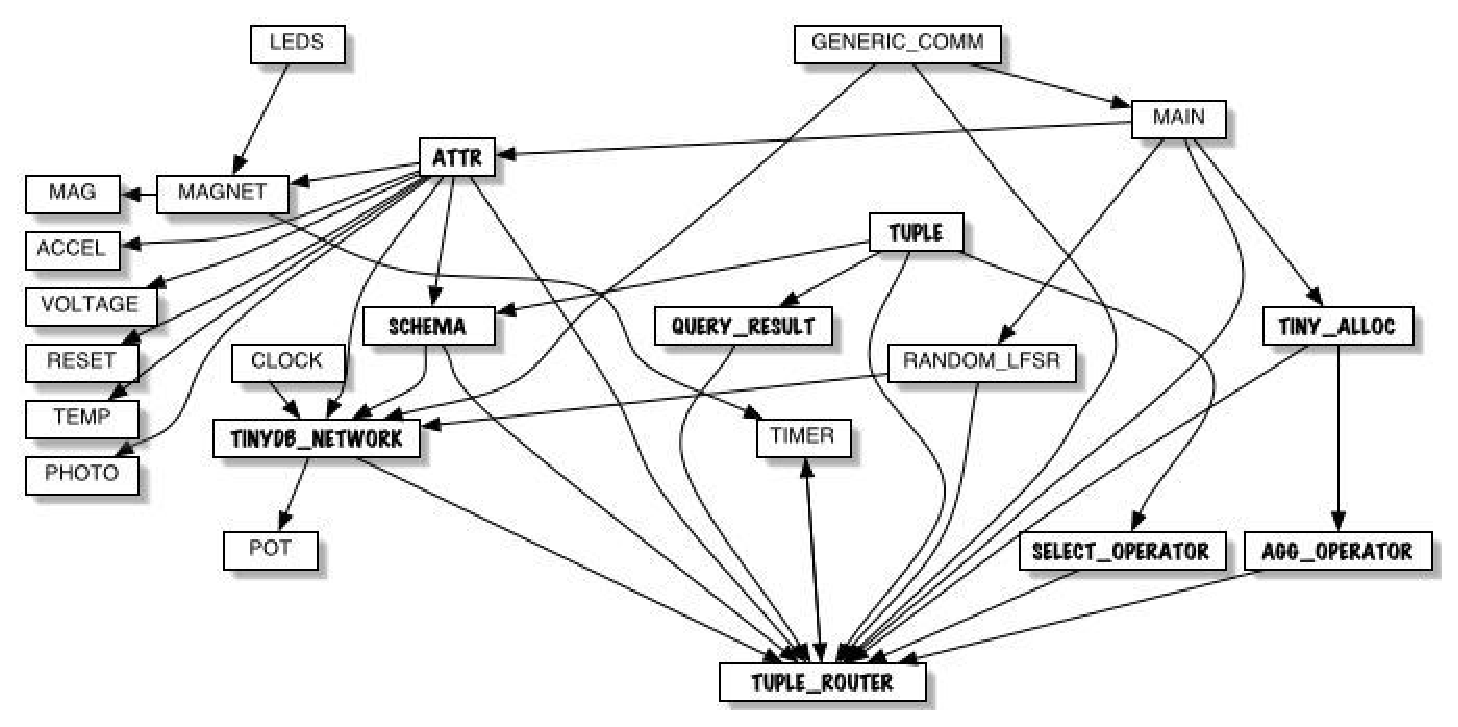
\psfig{file=circuit.eps,width=6in}
\caption{Component\index{component} diagram.  TinyDB\index{TinyDB}-specific components\index{component} are in the
  bold font.}
\label{fig:components}
\end{figure}

\subsection {The TinyDB\index{TinyDB} Sensor\index{sensor} Catalog\index{catalog} and Schema\index{schema} Manager}
\label{sec:catalog}

A {\em schema\index{schema}} describes the capabilities of the motes\index{mote} in the system as a
single virtual, database ``table\index{table}''.  This table\index{table} can contain any number
of typed {\em attributes\index{attribute}}).  It can also contain handles to a set of
{\em commands}, much like ``methods'' in the Object-Relational\index{Object-Relational}
extensions to SQL\index{SQL}.

During query processing, sensor\index{sensor} readings from each mote\index{mote} are placed
into {\em tuples\index{tuple}}, which may be passed between motes\index{mote} for multi-hop~\index{hop}\index{multi-hop}
routing\index{routing} and/or aggregation\index{aggregation}, or which may be passed out the serial port\index{serial}
at the top of the network to the front-end\index{front-end} code.

\subsubsection{\tt SCHEMA\index{schema}}
\label{sec:schema}
The {\tt SCHEMA\index{schema}} component\index{component} contains the code to initialize a schema\index{schema},
add attributes\index{attribute} and commands to the schema\index{schema}, and find out about the
contents of the schema\index{schema}.

It also contains the code to invoke a schema\index{schema} command locally ({\tt
SCHEMA\_INVOKE\_COMMAND}), and to send a message to invoke schema\index{schema}
commands on other nodes\index{node} ({\tt INVOKE\_COMMAND\_MESSAGE}).

\subsubsection {\tt ATTR}
\label{sec:attr}
This simple component\index{component} initializes the schema\index{schema}
(Section~\ref{sec:schema}), adding to it a fixed set of known
accessors and schema\index{schema} commands.  

{\bf TIP ON EXTENSIONS:} \marginpar{Should this be a running feature?}
If additional attribute\index{attribute} components\index{component} are added to the system, they
should be added to the initialization code here to make it into the
schema\index{schema}.

\subsubsection{\tt TUPLE\index{tuple}}
This component\index{component} provides fairly straightforward utilities to manage the
{\tt TUPLE\index{tuple}} data structure.

\subsubsection {\tt QUERY\_RESULT}
This component\index{component} converts between {\tt TUPLE}s\index{tuple}, {\tt QUERY\_RESULT}s,
and byte-strings.  These data structures are all defined in {\tt
nest/tos/include/TinyDB\index{TinyDB}.h}.  Briefly, a {\tt TUPLE}\index{tuple} is a typed vector
of values, as in SQL\index{SQL}; a {\tt QUERY\_RESULT} holds a tuple\index{tuple} and some
metadata, including the query ID, an index into the result set, and an
epoch\index{epoch} number.

\subsubsection {\tt MAGNET}
This component\index{component} is basically a temporary hack to access readings from
the magnetometers on the Rene motes\index{mote}.  In general, device-specific code
is to be provided by the general-purpose TinyOS\index{TinyOS} libraries.
(Section~\ref{sec:devices}).


\subsection{TinyDB\index{TinyDB} Query Processing Operators}
\label{sec:qp}
% \subsubsection {\tt TUPLE\_READER}
\subsubsection {\tt TUPLE\_ROUTER}
This deceptively-named component\index{component} provides the main query processing
functionality on a mote\index{mote}.  As Figure~\ref{fig:components} makes clear,
{\tt TUPLE\_ROUTER} is at the heart of the TinyDB\index{TinyDB} system.  It is called
a tuple\index{tuple} ``router'' because it routes tuples\index{tuple} through a variety of {\em
local} query processing components\index{component}.
% in the spirit of {\em eddies}~\cite{eddies}.  
{\em This component\index{component} does not do network
routing\index{routing}!}  For information on network routing\index{routing} in TinyDB\index{TinyDB}, see the
component\index{component} {\tt TINYDB\_NETWORK} (Section~\ref{sec:tinydbnetwork}).

The {\tt TUPLE\_ROUTER} component\index{component} contains three main execution
paths:
\begin{itemize}
\item Handling of new query messages
\item Result computation and propagation (each time a clock event goes off)
\item Subtree result message handling
\end{itemize}
We discuss these in turn.

\vspace{1em}
\noindent{\bf Handling New Queries}\\
New queries arrive in a {\tt TUPLE\_ROUTER\_QUERY\_MESSAGE}.  Each query
  is assumed to be identified by a globally unique ID, which is
  generated by the Java\index{Java} front-end\index{front-end}.  Query
  messages contain a part of a query: either a single field (attribute\index{attribute}) to
  retrieve, a single selection\index{selection} predicate\index{predicate} to apply, or a single
  aggregation\index{aggregation} function to apply.  All the {\tt QUERY\_MESSAGE}s describing a
  single query must arrive before the router will begin routing\index{routing} tuples\index{tuple}
  for that query.

Once all the {\tt QUERY\_MESSAGES}s have arrived, the router calls
  {\tt parseQuery()} to generate a compact representation of the query in
  which field names have been replaced with field IDs that can be used
  as offsets into the sensors\index{sensor} local catalog\index{catalog} ({\tt SCHEMA}\index{schema}).
  
Given a {\tt parsedQuery}, the tuple router allocates space at the end
  of the query to hold a single, ``in-flight'' tuple\index{tuple} for that query --
  this tuple\index{tuple} will be filled in with the appropriate data fields as the
  query executes.
  
{\tt TupleRouter} then calls {\tt setSampleRate()} to start (or restart) the
  mote\index{mote}'s 32khz clock to fire at the appropriate data-delivery rate for
  all of the queries currently in the system.  If there is only one
  query, it will fire once per ``epoch\index{epoch}'' -- if there are multiple queries,
  it will fire at the GCD of the delivery intervals of all the queries.

\vspace{1em}
\noindent{\bf Tuple\index{tuple} Delivery}\\
Whenever a clock event occurs ({\tt TUPLE\_ROUTER\_TIMER\_EVENT}), the
  router must perform four actions:
\begin{itemize}

\item Deliver tuples\index{tuple} which were completed on the previous clock event
  ({\tt deliverTuplesTask}).  If the query contains an aggregate\index{aggregate},
  deliver the aggregate\index{aggregate} data from the aggregate\index{aggregate} operator;  if not,
  deliver the tuple\index{tuple} that was filled out during the last
  iteration. Reset the counters that  indicate when these queries
  should be fired again.
  
\item Decrement the counters for all queries.  Any queries whose
  counters reach 0 need to have data delivered.  Reset the
  expression\index{expression}-specific state for these queries (this is specific
  to the expressions\index{expression} in the queries -- {\tt MAX} aggregates\index{aggregate}, for instance,
  will want to reset the current maximum aggregate\index{aggregate} to some large
  negative number.)

\item Fetch data fields for each query firing this epoch\index{epoch}.  Loop
  through all fields of all queries, fetch them (using the {\tt SCHEMA\index{schema}}
  interface), and fill in the appropriate values in the tuples\index{tuple}
  on the appropriate queries.  
  
\item Route filled-in tuples\index{tuple} to query operators.  First route to
  selections\index{selection}, then the aggregate\index{aggregate} (if it exists).  If any selection\index{selection}
  rejects a tuple\index{tuple}, discard it.

\end{itemize}

\vspace{1em}
\noindent{\bf Neighbor\index{neighbor} Result Arrival}\\
  When a result arrives from a neighbor\index{neighbor} ({\tt TUPLE\_ROUTER\_RESULT\_MESSAGE}),
  it needs to be integrated into the aggregate\index{aggregate} values being computed
  locally.  If the result corresponds to an aggregate\index{aggregate} query, that result
  is forwarded into the {\tt AGG\_OPERATOR} component\index{component}, otherwise it is 
  simply forwarded up the routing\index{routing} tree towards the root\index{root}.

\subsubsection {\tt SELECT\_OPERATOR}
The {\tt SELECT\_OPERATOR} is responsible for relational\index{relational} {\em
selection\index{selection}}: testing whether tuples\index{tuple} match predicates\index{predicate} (in task {\tt
doFilter\index{filter}}). Currently, the only expressions\index{expression} supported are standard
arithmetic comparisons of attributes\index{attribute} with constants.

\subsubsection {\tt AGG\_OPERATOR}
This component\index{component} performs two SQL\index{SQL} features: {\tt GROUP BY}\index{Group By} and
aggregation\index{aggregation}.

The optional {\tt GROUP BY}\index{Group By} feature partitions the data by the value
of a (set of) attribute\index{attribute}(s).  Aggregate\index{aggregate} functions are computed for each
partition, over any attributes\index{attribute} {\em not} in the {\tt GROUP BY}\index{Group By} clause.  In
the absence of a {\tt GROUP BY}\index{Group By} expression\index{expression}, the aggregate\index{aggregate} is computed
over all tuples\index{tuple}.  As described in Section~\ref{sec:queries}, aggregate\index{aggregate}
results are updated once per ``epoch\index{epoch}''.

The code in this component\index{component} needs to (a) take readings from the current
node\index{node} ({\tt AGG\_OPERATOR\_PROCESS\_TUPLE}), (b) merge those readings
with sub-aggregates\index{aggregate} from the subtree ({\tt
AGG\_OPERATOR\_PROCESS\_PARTIAL\_RESULT}), and (c) return this node's\index{node}
sub-aggregate\index{aggregate} results up the tree ({\tt AGG\_OPERATOR\_NEXT\_RESULT}).
It also manages allocating aggregation\index{aggregation} state for each group\index{group} using the
{\tt TINY\_ALLOC} component\index{component} (Section~\ref{sec:tinyalloc}), and
provides a utility to reset the running aggregation\index{aggregation} state ({\tt
AGG\_RESET\_EXPR\_STATE}).

\subsection {{\tt TINY\_ALLOC}: The TinyDB\index{TinyDB} Memory Manager}
\label{sec:tinyalloc}
This component\index{component}, being very general-purpose, is located in {\tt
nest/tos/shared/TINY\_ALLOC.\{c,comp\}} for use by other applications.

TINY\_ALLOC is a simple, handle-based\index{handle} compacting memory manager.  It
allocates bytes from a fixed size frame and returns handles (pointers
to pointers) into that frame.  Because it uses handles, TINY\_ALLOC can
move memory around in the frame without changing all the external
references.  Moving memory is a good thing because it allows frame
compacting and tends to reduce wasted space.  Handles can be accessed
via a double dereference (**), and a single dereference can be used
wherever a pointer is needed, but if a single dereference is to be
stored, the handle must be locked first (via {\tt TINY\_ALLOC\_LOCK}),
as otherwise TINY\_ALLOC may move the handle and make the reference invalid.

   Like all good TinyOS\index{TinyOS} programs, TINY\_ALLOC is split phase with
respect to allocation and compaction.  Allocation/reallocation
completion is signalled via a TINY\_ALLOC\_COMPLETE signal and
compaction via a TINY\_ALLOC\_COMPACT\_COMPLETE signal.  All other
operations complete and return in a single phase. Note that compaction
may be triggered automatically from allocation; in this case a
COMPACT\_COMPLETE event is not generated.

Handles\index{handle} are laid out in the frame as follows:
\begin{verbatim}
   [LOCKED][SIZE][user data] 

Where: 
    LOCKED     : a single bit indicating if the handle is locked 
    SIZE       : 7 bits representing the size of the handle 
    user data  : user-requested number of bytes (**h) points to
                 [user data], not [LOCKED].
\end{verbatim}
   Calling TOS\_COMMAND(TINY\_ALLOC\_SIZE(h)) returns the size of [user
data] (note that the internal function size() returns the size of the
entire handle, including the header byte.)

\subsection{TinyDB\index{TinyDB} Network Topology\index{topology} Manager}
\label{sec:tinydbnetwork}
The {\tt TINYDB\_NETWORK} component\index{component} handles all the mote-to-mote\index{mote} and mote-to-serial-port\index{serial}
communication for TinyDB\index{TinyDB}, routing\index{routing} {\em query} and {\em data} messages.
In doing so, it also participates in a distributed algorithm for
network topology\index{topology} layout.  Messages are all of type {\tt TOS\_Msg},
and begin with a {\tt DBMsgHdr} structure (see {\tt
nest/tos/include/TinyDB\index{TinyDB}.h}), followed by a payload.

\vspace{1em}
\noindent {\bf Topology\index{topology} Maintenance}\\ Most of the code in this
component\index{component} manages the network topology\index{topology}.  The network topology\index{topology} is
maintained as a routing\index{routing} {\em tree}, with Mote\index{mote} \#0 at the root\index{root}.  As a
rule, query messages flood down the tree in a straightforward fashion.
Data messages flow back up the tree, participating in more complex
query processing algorithms.  Mote\index{mote} \#0 passes result data to the
front-end\index{front-end} code via its serial\index{serial} interface.  The only exception to
``query-down/data-up'' rule is that the root\index{root} itself sends out periodic
(empty) data messages as a ``heartbeat''\index{heartbeat}, so that its communication
abilities can continue to be measured while a query runs.

By default, a simple tree-maintenance algorithm is used.  This
algorithm has each mote\index{mote} keep track of a list of other motes\index{mote} from which
it receives messages ({\em neighbors\index{neighbor}}).  Among these neighbors\index{neighbor}, it
chooses the best one as its {\em parent\index{parent}} in the tree.  Alternatively
(for testing purposes) the network can be forced to choose a static
topology\index{topology} based on the numbering of the nodes\index{node}.  This is done via the
{\tt TDB\_FORCE\_TOPOLOGY()} command.

\vspace{1em}
\noindent{\bf Message Handling}\\
Upon receiving a message on the network, this component\index{component} invokes the
internal routine {\tt processHeader}, which examines the header of
each packet received on the radio.  This code drives much of the logic
in the component\index{component}.  It first updates statistics that are maintained for
the parent-choice logic, and updates its choice of parent\index{parent} if
necessary.  Then, if the message is a data message destined for
another node\index{node}, it drops the message.  Otherwise, it handles the message
accordingly.

\subsection{TinyOS\index{TinyOS} Service Components\index{component}}
We describe these TinyOS\index{TinyOS} services only briefly.  For more detail see
TinyOS\index{TinyOS}.
\begin{itemize}
\item {\tt CLOCK}: Provides a system clock, and clock interrupts.
\item {\tt GENERIC\_COMM}: A generic communications layer, supporting
  radio and serial\index{serial} communication.
\item {\tt LEDS}: Control of the LED indicators on the motes\index{mote}.
\item {\tt MAIN}: A shell to initialize subordinate modules, and start
  them up.
\item {\tt POT}: Get and set the level of the potentiometer
  (transmission-power controller) on the radio.
\item {\tt RANDOM\_LFSR}: A psuedo-random number generator, based on a
  16-bit Linear Feedback Shift Register.
\item {\tt RESET}:  Reset a mote\index{mote} (eqivalent to toggling the 
power switch.)
\item {\tt TIMER}: A service for setting (multiple) timers to generate
  subsequent interrupts.
\end{itemize}

\subsection{Attributes\index{attribute}: Sensor\index{sensor} Components\index{component} and Introspection}
\label{sec:devices}
We describe these TinyOS\index{TinyOS} services only briefly.  For more detail see
TinyOS\index{TinyOS}.
\begin{itemize}
\item {\tt ACCEL}: Accelerometer: measures movement in two dimensions
  (X and Y).
\item {\tt MAG}: Magnetometer: measures magnetic field.
\item {\tt PHOTO}: Light sensor\index{sensor}.
\item {\tt TEMP}: Thermometer: measures temperature.
\item {\tt VOLTAGE}: Measures remaining voltage in the battery.
\end{itemize}
\section{Background}
\subsection{Related Reading}
\subsection{In-Network Processing\index{in-network}}
\subsection{Declarative Query Processing}

\section{Version History and Author Information}

\section{The TinyDB\index{TinyDB} License}

% Glossary entries
\nomenclature{\bf Active Messages (AM)}{A networking protocol developed at
  UC Berkeley, used for very-low-latency dispatch of incoming
  messages.  It provides an asynchronous (sometimes called
  ``split-phase'') programming model.}
\nomenclature{\bf Aggregation}{Aggregation is the process of
  bringing together multiple data objects.  In SQL, it typically
  denotes the summarization of multiple numeric values with a single
  summary statistic, like COUNT, AVERAGE, MAX or MIN.}
\nomenclature{\bf API}{Application Programming Interface.  A set of
  interfaces provided by a subsystem that enable programmers to use
  the subsystem in their own applications. }
\nomenclature{\bf Attribute}{In traditional databases, a row in a table,
  consisting of a name and a data type.  In TinyDB, an attribute often
  corresponds to a physical sensor reading like light, temperature,
  etc.  However, the system can support attributes provided in
  software as well, like NodeID, network parent, and so on.}
\nomenclature{\bf Catalog}{A set of metadata describing a database,
  including the schema, and whatever other metadata the system
  provides.}
\nomenclature{\bf Client}{In the TinyDB context, a piece of code running
  on a PC that invokes the TinyDB Java API.  Synonym for Front-End.}
\nomenclature{\bf Column}{See Attribute.}
\nomenclature{\bf COM1}{The name of the standard serial port on a PC.}
\nomenclature{\bf Component}{A basic building block in a TinyOS
  program. See the TinyOS documentation for details on the TinyOS
  programming model.}
\nomenclature{\bf Declarative Language}{A language in which you
  express what you desire, without detail on how to achieve it.
  Declarative languages are popular in database systems; SQL is
  (largely) declarative.  Declarative languages are useful for providing a
  very deep level of indirection between application requests and
  system implementation of the requests -- this is especially important if the
  system's optimal implementation could change frequently (as in a
  sensor network, which is quite unpredictable).}
\nomenclature{\bf Download}{In the context of TinyOS/TinyDB, this is the
  process of transfering a compiled code image onto a mote.}
\nomenclature{\bf Embedded C}{A program written in C that runs
  autonomously on a small device like a mote.} 
\nomenclature{\bf Epoch}{A discrete window of time.  In TinyDB's SQL, new
  answers to a query are produced every epoch, and the duration of an
  epoch can be specified in the query.}
\nomenclature{\bf Expression}{A simple interpretable clause in a query,
  like an arithmetic comparison (e.g.\ {\tt light $>$ 80}), or an
  aggregate function (e.g.\ {\tt AVERAGE(temp)})}.
\nomenclature{\bf Filter}{A predicate that may remove some readings from
  the query.  Synonym for Selection.}
\nomenclature{\bf Front-End}{In the TinyDB context, a piece of code running
  on a PC that invokes the TinyDB Java API.  Synonym for Client.}
\nomenclature{\bf Group By}{In SQL, an expression that partitions the set of
  tuples that satisfy a query, to prepare for computation of an
  aggregate per partition.  Typically the Group By expression is
  simply an attribute name, e.g.\ {\tt GROUP BY temp}; tuples are
  partitioned by the value of the attribute.}
\nomenclature{\bf GUI}{Graphical User Interface.}
\nomenclature{\bf Handle}{A pointer to a pointer to an object.  The
  double level of indirection allows the objects to be relocated
  without informing the code that manipulates the handles.}
\nomenclature{\bf Heartbeat}{A periodic network message that simply
  indicates that the sender is active and connected.}
\nomenclature{\bf In-Network}{A description for algorithms that run in
  intermediate network devices in a multi-hop network, rather than the
  hosts at the endpoints.}
\nomenclature{\bf Listener}{A Java object that responds to certain
  kinds of events.}
\nomenclature{\bf Mote (Berkeley Mote)}{A wireless sensor network
  node, developed at UC Berkeley.  A mote is a device combining a small
  microprocessor, one or more sensors, and a radio.  The name ``mote''
  comes from the ``Smart Dust'' metaphor introduced by sci-fi author Neal Stephenson.}
\nomenclature{\bf Multi-Hop}{A scenario in which network messages
  visit multiple routers between source and destination.}
\nomenclature{\bf Neighbor}{Two network nodes are neighbors if they
  can communicate directly, without involving any intermediate routing.}
\nomenclature{\bf Node}{In this context, a compute device in a
  network; typically a mote in a sensor network.}
\nomenclature{\bf Object-Relational}{A database model developed in the
  Postgres project at UC Berkeley, which extends the
  relational model with object-oriented features like extensible
  abstract data types, including OO methods that are executed by the
  database engine (rather than at a client).}
\nomenclature{\bf Parent}{In a TinyDB routing tree, the parent of node
  $n$ is the node that listens to $n$'s data messages.}
\nomenclature{\bf Predicate}{A boolean expression.}
\nomenclature{\bf Processed}{In the TinyDB API, a result tuple is considered
  ``processed'' when all the attributes have been concatenated
  together with fully aggregated values.}
\nomenclature{\bf
  Ptolemy}{\htmladdnormallink{Ptolemy}{http://ptolemy.eecs.berkeley.edu}
  is a simulation project at UC Berkeley.  The TinyDB application
  borrows a small piece of code from 
  Ptolemy for plotting results.} 
\nomenclature{\bf Query Plan}{An interpretable description for
  executing a query, typically consisting of a few high-level
  operators connected in a dataflow tree.}
\nomenclature{\bf Query Processor}{A system for executing queries.}
\nomenclature{\bf Relational Model, Relational Languages}{Invented by
  Turing Award-Winner Ted Codd, the
  relational data model is the most prevalent representation for data
  today.  It is extremely simple, representing all information as
  relations (``tables'') consisting of tuples (``rows'') made up of
  well-typed attributes (``columns'').  A relational query language is
  one that can express a subset of 1st-order logic over relations.
  The standard relational query language is SQL.}
\nomenclature{\bf Root}{In TinyDB, this refers to the root of the
  routing tree, which is a sensor that is connected to the serial port
  of the PC running the front-end code.}
\nomenclature{\bf Routing}{The process of moving data through a
  multi-hop network from source to destination.  In TinyDB, the
  dataflow involved in routing interacts significantly with the
  dataflow involved in query processing.}
\nomenclature{\bf Row}{See Tuple.}
\nomenclature{\bf Sample}{In the sensor context, this often refers to
  a single discrete reading taken by a sensor.  It is called a sample to highlight
  the approximate nature of representing a continuous, real-world
  process as a stream of discrete digital readings.}
\nomenclature{\bf Schema}{A metadata description of a relation or set of
  relations.  A simple schema includes the name of the relation(s), the
  names and data types of the attributes in the relation, and the
  default order of the attributes.  Note that the schema describes
  what data {\em can} exist in the relation, not what {\em currently}
  exists.}
\nomenclature{\bf Selection}{In relational languages, the operation of
  choosing those tuples in a relation that match some predicate.  See Filter.}
\nomenclature{\bf Semantics}{The meaning of a construct.}
\nomenclature{\bf Sensor}{A device for converting physical phenomena into
     electronic signals.  In this document we sometimes use the word sensor
     interchangeably with the word mote: the combination of a sensor, a
     processor, and a radio.}  
\nomenclature{\bf Sensor Network}{A network -- often a wireless
  network -- in which the nodes are devices like motes that combine
  sensors with processing and commmunication.}
\nomenclature{\bf Serial Port}{An I/O port present on most PCs.}
\nomenclature{\bf SQL}{The Structured Query Language, a standard
	  language used for specifying queries to relational databases.}
\nomenclature{\bf Table}{See Relation.}
\nomenclature{\bf Timeslot}{An assigned range of time.  In order to
  avoid network congestion, some protocols explicitly allocate timeslots across
  potential senders so that their messages do not collide.}
\nomenclature{\bf TinyDB}{A system for declaring and executing queries
  in a wireless sensor network.}
\nomenclature{\bf TinyOS}{A set of C-based low-level libraries for writing
  embedded systems on the Berkeley Motes.  Key features of TinyOS
  include hardware abstractions for the Berkeley motes, an
  Active Messages-based communication layer for both radio and serial
  communication, and a programming model that supports both procedure
  calls and asynchronous event programming.}
\nomenclature{\bf Topology}{In our discussion, the directed graph that
  represents the communication pattern between motes in a wireless network.}
\nomenclature{\bf Tuple}{A list of attribute-value pairs that
  corresponds to the schema of some relation.}
\printindex
\printglossary
\end{document}
